%%%%%%%%%%%%%%%%%%%%%%%%%%%%%%%%%%%%%%%%%%%%%%%%%%%%%%%%%%%%%%%%%%%%%%%%%%%%%%%%%%%%%%%%%
%%%%%%%%%%%%%%%%%%%%%%%%%%%%         CONCEPTUAL DESIGN         %%%%%%%%%%%%%%%%%%%%%%%%%%
%%%%%%%%%%%%%%%%%%%%%%%%%%%%%%%%%%%%%%%%%%%%%%%%%%%%%%%%%%%%%%%%%%%%%%%%%%%%%%%%%%%%%%%%%

\section{Conceptual Design Approach} % (20 Points)
\label{sec:ConceptualDesign}
% Section Requirements:
% 1) Decomposition of mission requirements into subsystem requirements.
% 2) Preliminary design / sizing results; concept sketch, if available (does not have to be representative of the final design) 
% 3) Sensitivity Study of Design Parameters



%%%%%%%%%%%%%%%%%%%%%%%%%%%%%
%%%% - subsystem Reqs - %%%%
%%%%%%%%%%%%%%%%%%%%%%%%%%%%%
\subsection{Mission Requirements Decomposition}
\label{ssec:MissionReqs}

We decompose the mission requirements into subsystem requirements in \cref{tab:reqdecomp}. We include the score equations in the second table column, and define the variables as part of the mission requirements stated in column 3. In column 4, we list the decomposed subsystem requirements. For the sake of brevity, we did not include the take-off distance requirement of 25 ft that applies to all FM. Also for the sake of brevity, we present the subsystem decompositions in column 4 cumulatively, for example, items that are listed for FM1 also apply to FM2 and FM3.


% {\(\text{GM score} = t_{\mathrm{min}} / t_{N}\)} where \(t_{\mathrm{min}}\) is the fastest time of all teams, and \(t_{N}\) is our time to load the full M2 payload, unload the M2 Payload, Load the M3 Payload, and deploy the M3 payload. 
% {\(\text{FM1 score} = 1.0\)} when successfully taking off within 25 ft, flying 3 laps, within a 5-minute window, followed by a safe landing. M1 is completed without payload, but with all deployment mechanisms.
% {\(\text{FM2 score} = 1 + (N_s/t) / (N_s/t)_{max}\)} where \(N_s\) is the number of syringes carried, and \(t\) is the time taken to take off within 25 ft, fly 3 laps, within a 5 minute maximum time window, followed by a safe landing. 
% {\(\text{FM3 score} = 2 + Npd/Npd_{max}\)} where \(Npd\) is the number of payload deployments within a 10 minute window, following the pattern: take off within 25 ft, fly 1 lap, land successfully, taxi to drop-off area, deploy 1 Vial Package, taxi to runway, repeat, all without tripping any of the package shock sensors. Where \(Npd \leq N_s/10\). 
% For both M2 and M3 \(max\) indicates the maximum score ratio among all teams.

% \subsubsection{Aerodynamics Requirements}
% \label{sssec:AerodynamicReqs}

% The major requirements for the aerodynamics subsystem are: Maximize aerodynamic efficiency in order to use less energy to overcome drag for all flight missions.  Design the wing loading to be able to take off and fly with design max payload weight.  Keep the airframe within the maximum of 8 linear feet.  Design for a stall speed that will allow takeoff within 25 ft.

% \subsubsection{Structural Requirements}
% \label{sssec:StructuralReqs}

% The breakdown of mission requirements for the structures subsystem include: Minimize the structural weight while maintaining sufficient rigidity to keep the aerodynamics as designed, especially when full payload weight is in use; ensure the structure is sufficiently rigid to avoid aerodynamic flutter within the flight envelope; and provide sufficient dampening upon landing to protect the payload from greater than 5g impulses.

% \subsubsection{Propulsion Requirements}
% \label{sssec:PropulsionReqs}

% The propulsion subsystem requirements are to: Have sufficient system efficiency and battery capacity to enable completion of FM 1. Maximize speed with sufficient endurance to maximize scores for FM 2 and FM 3. Provide sufficient thrust for a take-off distance less than or equal to 25 feet.

% \subsubsection{Payload System Requirements} %change this to be specifically what it is (like bomb drop or whatever the specific mission is)
% \label{sssec:SpecialReqs}

% The payload subsystem requirements include: Provide a fuselage structure to encapsulate and retain both M2 and M3 payloads while minimizing structural weight. Include automated vial package deployment without inducing a greater than 5g shock.  Design a method to account for the adjusted center of gravity associated with every deposited vial package during FM3.

\begin{table}[h!]
	\centering
	\caption{Mission scores and requirements decomposed into subsystem requirements.}
	\label{tab:reqdecomp}
	\rowcolors{2}{BYUbluelite}{white}
	\begin{tabular}{ p{.25in} ? C{.75in} ? p{2.35in} ? p{3.5in} }
		
		\rowcolor{BYUbluemid}
		
		\cellcolor{white} & Score Eqn. & Mission Requirements & Subsystem Requirement Decomposition   \\
		
		GM & \(\cfrac{t_{min}}{t_n}\) & \thead{\tabitem Manually load and unload FM2 payload\\\tabitem Manually load, and auto-deposit, FM3 payload\\\tabitem Complete in time, \(t_n\)} & \thead{\tabitem Intuitive and accessible fuselage design\\\tabitem Simple, quick, gentle, and reliable package deposition capabilities} \\
		
		FM1 & \(1.0\) & \thead{\tabitem Complete 3 laps within 5 minutes\\\tabitem Carry empty payload management hardware} & \thead{\tabitem Wing and propulsion design capable of \(\leq\)25ft take-off\\\tabitem Efficiency in all systems to allow \(>\)3 laps in \(<\)5 minutes}\\
		
		FM2 & \( 1 + \frac{N_s/t}{[N_s/t]_{max}}\) & \thead{\tabitem Complete 3 laps in \(t\leq5\) minutes\\\tabitem Carry \(N_s\geq10\) syringes} & \thead{\tabitem Strong, lightweight wing structure to carry heavy payload\\\tabitem Fuselage volume large enough to carry maximum \(N_s\) \\\tabitem High propulsion system thrust to maximize flight speed\\\tabitem Low wing lift coefficient at cruise, also to maximize flight speed \\\tabitem Wing, tail, and control surface rigidity to prevent flutter at high speed}\\
		
		FM3 & \(2 + \frac{N_{vd}}{[N_{vd}]_{max}}\) & \thead{\tabitem Carry vial packages \(N_v \geq N_{vd} \leq N_s/10\) \\\tabitem Deposit 1 of \(N_{vd}\) total delivered packages each lap\\\tabitem DO NOT trip shock sensors} & \thead{\tabitem Wing stall speed low enough to not trip sensors due to take-off acceleration\\\tabitem Structure and landing gear capable of damping landing forces on payload \\\tabitem Payload management system that maintains aircraft static stability\\\tabitem Propulsion and control surfaces designed for on-ground agility.}\\
		
	\end{tabular}
\end{table}



%%%%%%%%%%%%%%%%%%%%%%%%%%%%%%%%%%%%%
%%% - Preliminary Design/Sizing - %%%
%%%%%%%%%%%%%%%%%%%%%%%%%%%%%%%%%%%%%
\subsection{Preliminary Design}
\label{ssec:PreliminaryDesign}

%%%%%%%%%%%%%%%%%%%%%%%%%%%%%
%%%% - Concept Sketch - %%%%
%%%%%%%%%%%%%%%%%%%%%%%%%%%%%
%3 drawing views and rendered view of latest CAD models:  Make sure the aspect ratios match the draft figure names.


%Preliminary design / sizing results

After utilizing Pugh matrices to aid in configuration selection for our aircraft, we arrived at the configuration seen in \cref{fig:render}.
Namely: a single high mount wing, dual tractor rotors, single boom, and conventional tail design.
Using common hand calculation formulas\footnote{see \textit{Flight Vehicle Design}, by Dr. Andrew Ning, \url{https://scholarsarchive.byu.edu/cgi/viewcontent.cgi?article=1027&context=books}} and XFLR5 software, we arrived at a conceptual design with the following specifications: a fuselage diameter and length of  7 in.~and  4 ft, respectively, a wing span of 8 ft, an aspect ratio of 7.1, a wing loading of 1.67 lbs/ft$^2$, horizontal and vertical tail volume ratios of 0.82 and 0.06, respectively, a stall velocity of 32.4 ft/s, and a take-off distance of 18.2 ft. We have also initiated the setup of some of our preliminary design trades, simulations, and analyses; for example \cref{fig:vpm} shows a preliminary look at rotor-on-wing interactions using a vortex particle method.\footnote{\url{https://github.com/byuflowlab/FLOWUnsteady}}

Our current concept includes a section of the fuselage we call the ``payload manager'' which we will design to lower and release the vial packages one at a time.  The payload manager will contain the vial packages suspended by elastic chords to absorb the acute accelerations produced by takeoff, turbulence, and landing.  After a signal from the pilot, the payload manager will lower slowly to the ground by a motor-powered pulley system, and the elastic chord around one of the packages will be released by a servo, leaving the package safely on the ground. The package manager will then rise back to its stowed position and the aircraft will proceed with another flight sequence.  In order to maintain static and dynamic stability, we will release the rear and front most packages in an alternating sequence, beginning with the rear most. This will shift the center of gravity (c.g.) forward by approximately half the width of a package (1.25 in.), then back to its original position when the front most package is released.  We will design our airframe with both c.g. flight states in mind to ensure a stable aircraft throughout FM3.

\begin{figure}[h!]
	\centering
	\begin{subfigure}[t]{0.475\textwidth}
		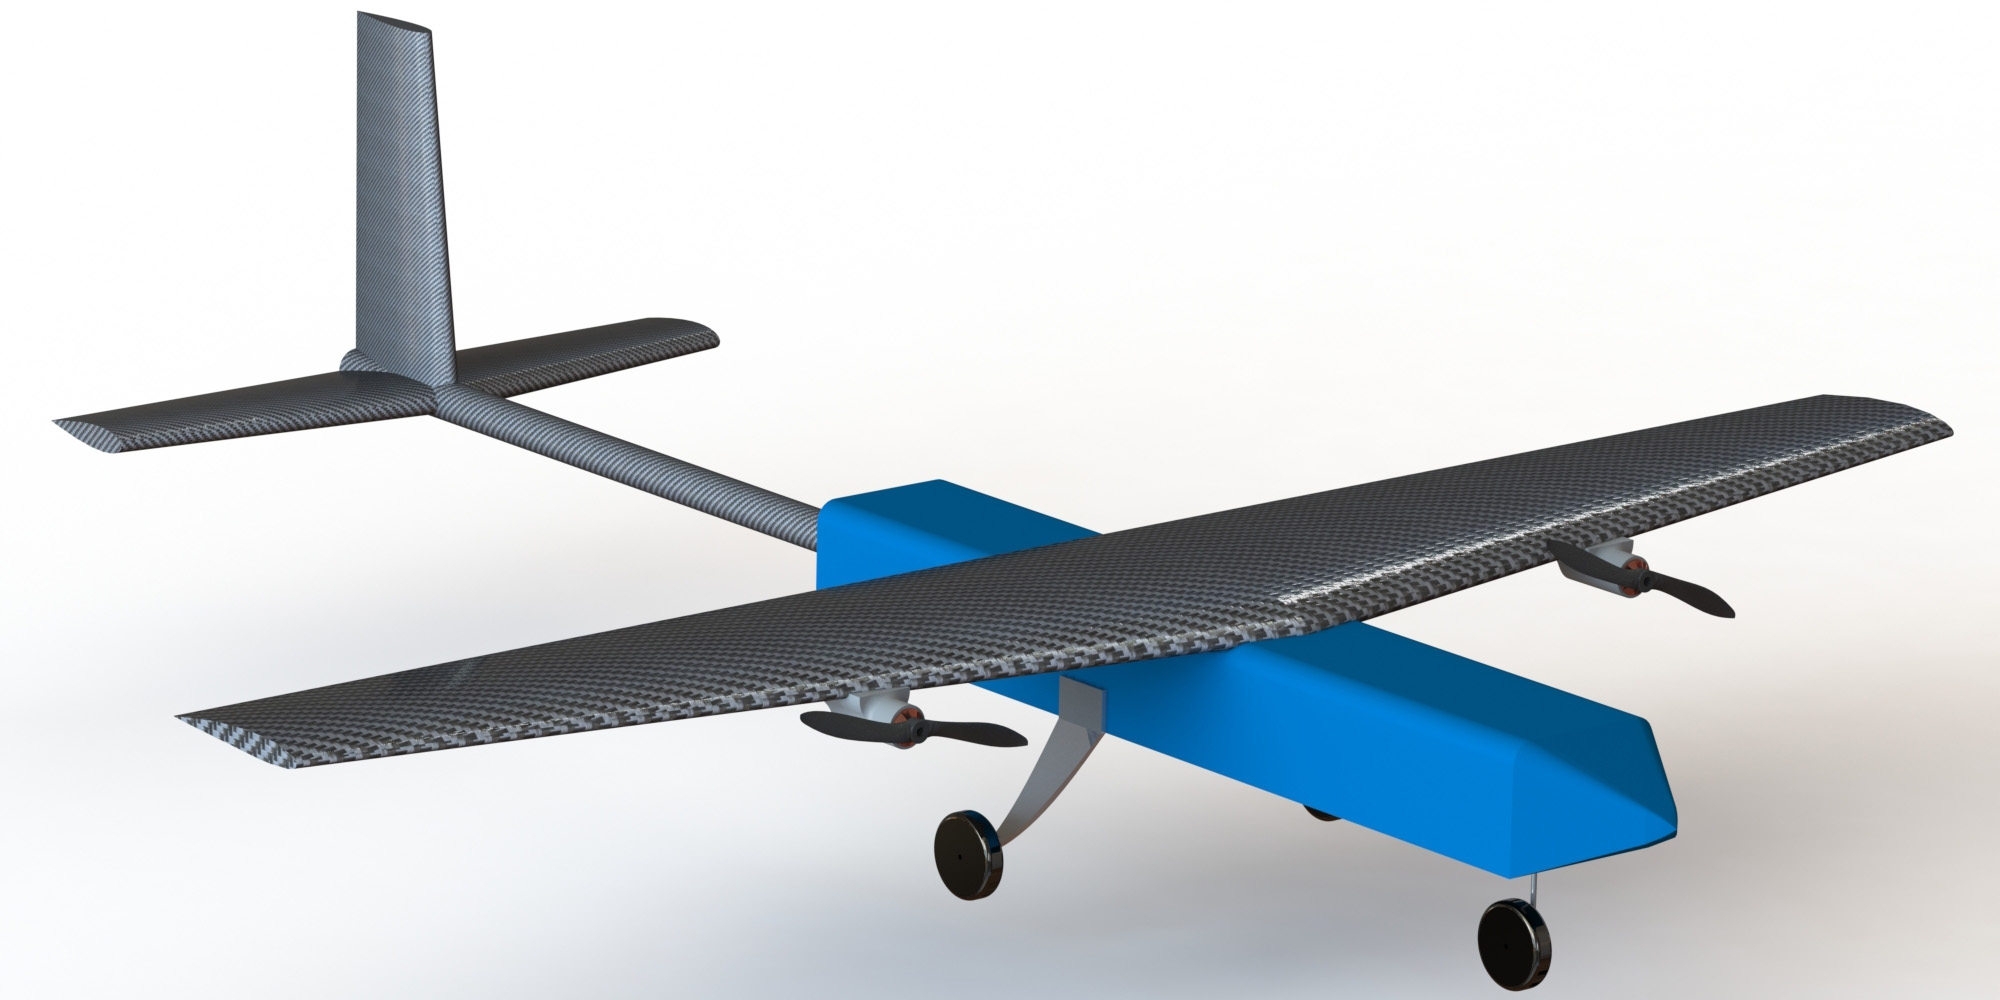
\includegraphics[width=\textwidth]{figures/render.JPG}
		\caption{Rendered view of concept CAD}
		\label{fig:render}
	\end{subfigure}
	%
	\begin{subfigure}[t]{0.475\textwidth}
		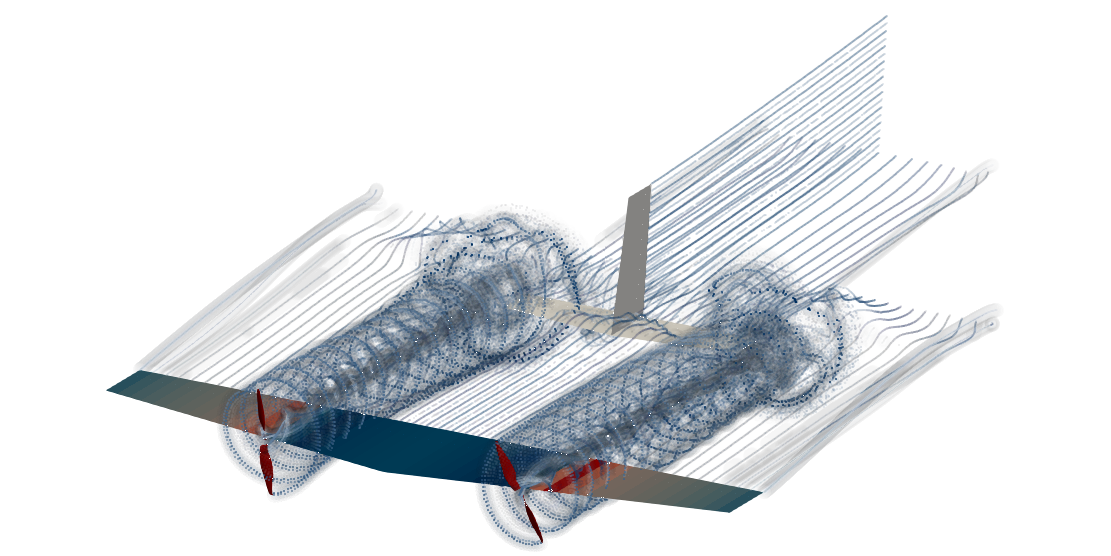
\includegraphics[width=\textwidth]{figures/vpmprelimsmall.png}
		\caption{Preliminary simulation using a vortex particle method to capture the near wake rotor-on-wing effects}
		\label{fig:vpm}
	\end{subfigure}
	% 	\begin{subfigure}[b]{0.475\textwidth}
	% 		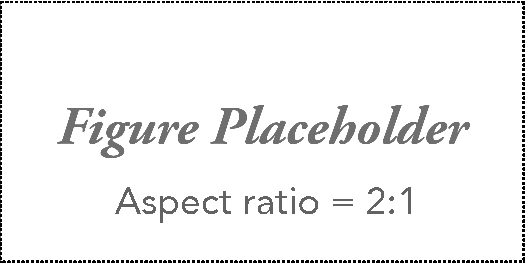
\includegraphics[width=\textwidth]{draft2x1}
	% 		\caption{Front View}
	% 		\label{fig:frontview}
	% 	\end{subfigure}
	% 	%
	% 	\begin{subfigure}[b]{0.475\textwidth}
	% 		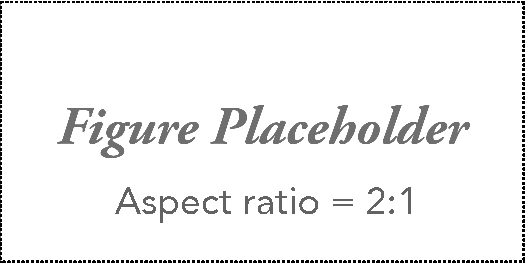
\includegraphics[width=\textwidth]{draft2x1}
	% 		\caption{Rendered View}
	% 		\label{fig:renderedview}
	% 	\end{subfigure}
	\caption{Visualizations of our conceptual design.}
	\label{fig:conceptimages}
\end{figure}
%%%%%%%%%%%%%%%%%%%%%%%%%%%%%%%
%%%% - Sensitivity Study - %%%%
%%%%%%%%%%%%%%%%%%%%%%%%%%%%%%%
\subsection{Sensitivity Study}
\label{ssec:SensitivityStudy}

%Figure related to sensitivity study, move around to get formatting correct...

For our sensitivity study, we first differentiated between design variables that could increase/decrease our score and those that were only related to the minimum requirements. We found the parameters that could affect the score to be: wing area, aircraft empty weight (including batteries), total lap distance, number of payload units, and available power.  To perform our study, we took these parameters and ran them through common hand calculations to find the mission objective scores. In order to normalize the scores as done in the competition, we ran the analysis first without normalization, from which we saved the maximum scores. We then used those maxima as the normalization factors and re-ran the analysis. We found (as shown in \cref{fig:sensitivity}) that the wing area and parasitic drag (not plotted) had the same sensitivities, thus we want to minimize drag and maximize wing loading (while still being able to take off).  The available power was also important, and can be affected by battery capacity, discharge rate, voltage, and system efficiency. Interestingly, the lap distance is highly sensitive, thus we want to minimize turn radius. Obviously the number of payload units in FM2 and FM3 highly effect the overall score.  We should also note that the aircraft empty weight had a relatively negligible effect on the overall sensitivity, but is important to keep in mind when designing for a feasible aircraft.